\documentclass[14pt, a4paper]{extarticle}
\usepackage{GOST}
\usepackage{array}
\usepackage{verbatim}
\usepackage[detect-all]{siunitx}
\usepackage{amsmath}
\usepackage{amssymb}
\usepackage[utf8]{inputenc}
\usepackage{hyperref}

\usepackage{ifthen}


\usepackage{tempora}


\makeatletter
\renewcommand\@biblabel[1]{#1.}
\makeatother

% Для листинга кода:
\usepackage{listings}
\lstset{ %
	language=python,                 % выбор языка для подсветки (здесь это С)
	basicstyle=\small\sffamily, % размер и начертание шрифта для подсветки кода
	numbers=left,               % где поставить нумерацию строк (слева\справа)
	numberstyle=\tiny,           % размер шрифта для номеров строк
	stepnumber=1,                   % размер шага между двумя номерами строк
	numbersep=5pt,                % как далеко отстоят номера строк от подсвечиваемого кода
	showspaces=false,            % показывать или нет пробелы специальными отступами
	showstringspaces=false,      % показывать или нет пробелы в строках
	showtabs=false,             % показывать или нет табуляцию в строках
	frame=single,              % рисовать рамку вокруг кода
	tabsize=2,                 % размер табуляции по умолчанию равен 2 пробелам
	captionpos=t,              % позиция заголовка вверху [t] или внизу [b] 
	breaklines=true,           % автоматически переносить строки (да\нет)
	breakatwhitespace=false, % переносить строки только если есть пробел
	escapeinside={\#*}{*)}   % если нужно добавить комментарии в коде
}


%для графиков
\usepackage{pgfplots}
\usepackage{filecontents}
\usetikzlibrary{datavisualization}
\usetikzlibrary{datavisualization.formats.functions}

\begin{document}
	
	\begin{table}[ht]
		\centering
		\begin{tabular}{|c|p{400pt}|} 
			\hline
			\begin{tabular}[c]{@{}c@{}} 
\includegraphics[scale=1]{baum.jpg} \\\end{tabular} &
			\footnotesize\begin{tabular}[c]{@{}c@{}}\textbf{Министерство~науки~и~высшего~образования~Российской~Федерации}\\\textbf{Федеральное~государственное~бюджетное~образовательное~учреждение}\\\textbf{~высшего~образования}\\\textbf{«Московский~государственный~технический~университет}\\\textbf{имени~Н.Э.~Баумана}\\\textbf{(национальный~исследовательский~университет)»}\\\textbf{(МГТУ~им.~Н.Э.~Баумана)}\\\end{tabular}  \\
			\hline
		\end{tabular}
	\end{table}
	\noindent\rule{\textwidth}{4pt}
	\noindent\rule[14pt]{\textwidth}{1pt}
	\hfill 
	\noindent
	\makebox{ФАКУЛЬТЕТ~}%
	\makebox[\textwidth][l]{\underline{~«Информатика и системы управления»~~~~~~~~~~~~~~~~~~~~~~~~~~~~~~~~~}}%
	\\
	\noindent
	\makebox{КАФЕДРА~}%
	\makebox[\textwidth][l]{\underline{~«Программное обеспечение ЭВМ и информационные технологии»~}}%
	
	
	\begin{center}
		\vspace{1.5cm}
		{\bf\huge Отчёт\par}
		{\bf\Large по лабораторной работе № 1\par}
		\vspace{0.7cm}
	\end{center}
	
	
	\noindent
	\makebox{\large{\bf Название:}~~~}
	\makebox[\textwidth][l]{\large\underline{Изучение функции распределения~~~~~~~~~~~~~~~~~~~~}}
	\makebox[\textwidth][l]{\large\underline{ и функции плотности распределения случайных чисел.~~~~~~~~~~~~~~~~~}}
	
	\noindent
	\makebox{\large{\bf Дисциплина:}~~~}
	\makebox[\textwidth][l]{\large\underline{~Моделирование~~~~~~~~~~~~~~~~~~~~~~~~~~}}\\
	
	\vspace{1.5cm}
	\noindent
	\begin{tabular}{l c c c c c}
		Студент      & ~ИУ7-75Б~               & \hspace{2.5cm} & \hspace{2cm}                 & &  Д.В. 
		Сусликов \\\cline{2-2}\cline{4-4} \cline{6-6} 
		\hspace{3cm} & {\footnotesize(Группа)} &                & {\footnotesize(Подпись, дата)} & & {\footnotesize(И.О. Фамилия)}
	\end{tabular}
	
	\noindent
	\begin{tabular}{l c c c c}
		Преподаватель & \hspace{5cm}   & \hspace{2cm}                 & & ~~~~~~И.В. Рудаков~~~~~~\\\cline{3-3} \cline{5-5} 
		\hspace{3cm}  &                & {\footnotesize(Подпись, дата)} & & {\footnotesize(И.О. Фамилия)}
	\end{tabular}
	
	\vspace{0.6cm}
	\begin{center}	
		\vfill
		\large \textit {Москва, 2021}
	\end{center}
	
	\thispagestyle {empty}
	\pagebreak
	
	% СОДЕРЖАНИЕ 
	\clearpage
		
	% ВВЕДЕНИЕ
	\clearpage
	\section{Задание}
	\addcontentsline{toc}{section}{Задание}
	Требуется исследовать следующие 2 распределения:
	\begin{itemize}
		\item[1)] равномерное распределение;
		\item[2)] распределение Пуассона.
	\end{itemize}
	Для данных распределений построить графики функций распределений и функций плотности распределения случайных чисел. 
	\newpage
	
	
	\section{Теория}
	\addcontentsline{toc}{section}{Теория}
	
	\textbf{Равномерное распределение }
		
	Функция распределения:
	
	\begin{equation*}
		F_X(x) \equiv P(X \le x) = \left\{
		\begin{matrix}
			0, & x < a \\
			\dfrac{x-a}{b-a}, & a \le x < b \\
			1, & x \ge b
		\end{matrix}
		\right.
	\end{equation*}

	Плотность распределения:
	
	\begin{equation*}
		f_X(x) = \left\{
		\begin{matrix}
			{1 \over b-a}, & x\in [a,b] \\
			0, & x\not\in [a,b]
		\end{matrix}
		\right.
	\end{equation*}
	
	
	\textbf{Пуассоновское распределение}
	
	Функция распределения:
	
	\begin{equation*}
		F(x) =  \frac{\Gamma(|k + 1), \mu)}{|k|!}
	\end{equation*}

	Плотность распределения:
	
	\begin{equation*}
		f(x) = \frac{\mu^{k}}{k!} e^{-\mu} 
	\end{equation*}	
	\newpage
	
	\section{Результаты работы}
	\addcontentsline{toc}{section}{Задание}
	
	\begin{figure}[h]
		\centering{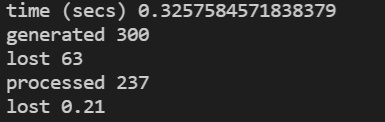
\includegraphics[scale=0.8]{source/1.png}}
		\centering\caption{График функции распределения и плотности распределения равномерной случайной величины при a = -5, b = 5}
	\end{figure}
	
	\newpage
	
	\begin{figure}[h]
		\centering{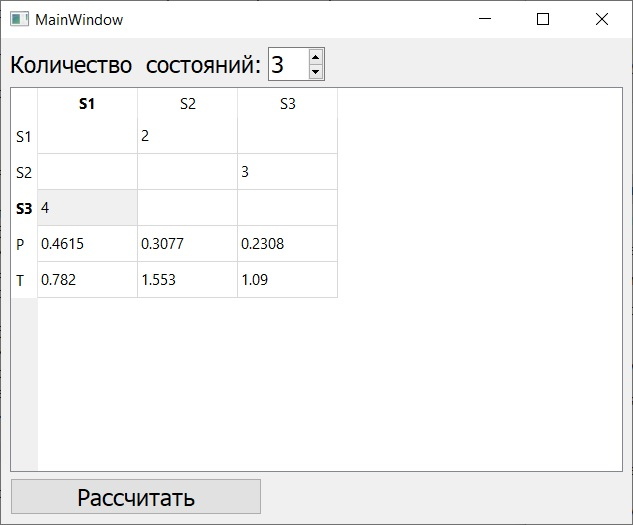
\includegraphics[scale=0.8]{source/11.png}}
		\centering\caption{График функции распределения и плотности распределения равномерной случайной величины при a = 0, b = 5}
	\end{figure}
	
	\newpage
	
	\begin{figure}[h]
		\centering{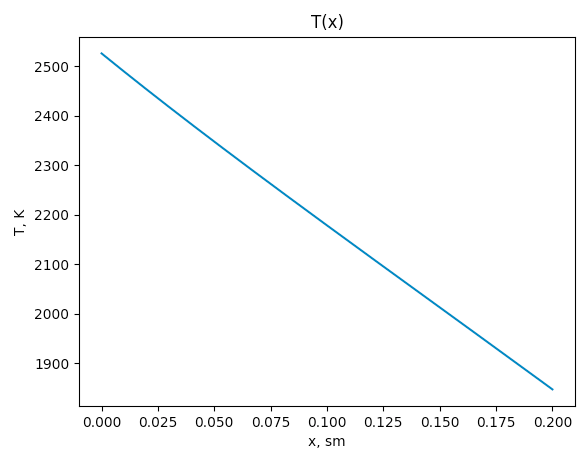
\includegraphics[scale=0.8]{source/2.png}}
		\centering\caption{График функции распределения и плотности распределения Пуассона при $\mu$ = 10 в интервале от -1 до 20}
	\end{figure}
	
	\newpage
	
	\begin{figure}[h]
		\centering{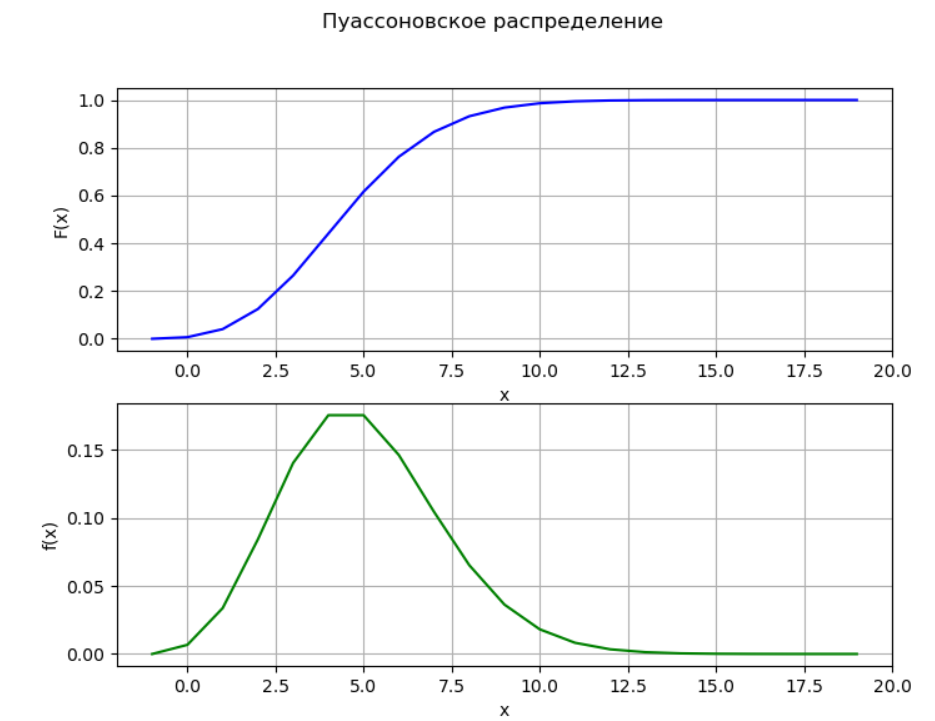
\includegraphics[scale=0.8]{source/22.png}}
		\centering\caption{График функции распределения и плотности распределения Пуассона при $\mu$ = 5 в интервале от -1 до 20}
	\end{figure}

	
	
	\newpage
	\textbf{Текст программы}
	\begin{lstlisting}
		import matplotlib.pyplot as plt
		from scipy.stats import poisson
		import numpy as np
		
		def uniform_distribution(a, b, x):
			if (x < a):
				return 0
			elif (x >= b):
				return 1
			else:
				return (x - a) / (b - a)
		
		def uniform_density(a, b, x):
			if (a <= x <= b):
				return 1 / (b - a)
			else:
				return 0
		
		
		def poisson_distribution(x, mu):
			return poisson(mu).cdf(x)
		
		
		def poisson_density(x, mu):
			return poisson(mu).pmf(x)
		
		def draw_graphs(x, y_distribution, y_density, name):
			fig, axs = plt.subplots(2, figsize=(8, 6))
			
			fig.suptitle(name)
			axs[0].plot(x, y_distribution, color='blue')
			axs[1].plot(x, y_density, color='green')
			
			axs[0].set_xlabel('x')
			axs[0].set_ylabel('F(x)')
			
			axs[1].set_xlabel('x')
			axs[1].set_ylabel('f(x)')
			
			axs[0].grid(True)
			axs[1].grid(True)
			plt.show()
		
		def main():
			a = float(input("Input a: "))
			b = float(input("Input b: "))
			
			delta = b - a
			x = np.arange(a - delta / 2, b + delta / 2, 0.001)
			
			y_distribution = [uniform_distribution(a, b, _x) for _x in x]
			y_density = [uniform_density(a, b, _x) for _x in x]
			draw_graphs(x, y_distribution, y_density)
			
			mu = float(input("Input mu: "))    
			x = np.arange(-1, 20)
			y_distribution = poisson_distribution(x, mu)
			y_density = poisson_density(x, mu)
		
			draw_graphs(x, y_distribution, y_density)
		
		if __name__ == '__main__':
			main()
	\end{lstlisting}	
\end{document}